%%%%%%%%%%%%%%%%%%%%%%%%%%%%%%%%%%%%%%%%%%%%%%%%

% Specify the command that you want into the header of the
% index.md file

%%%%%%%%%%%%%%%%%%%%%%%%%%%%%%%%%%%%%%%%%%%%%%%%

% Options for packages loaded elsewhere
\PassOptionsToPackage{unicode}{hyperref}
\PassOptionsToPackage{hyphens}{url}
\PassOptionsToPackage{dvipsnames,svgnames*,x11names*}{xcolor}
%
\documentclass[
  12pt,
  oneside]{report}
%%\usepackage{lmodern}
%
% Set line spacing
\usepackage{setspace}
\setstretch{1.5}

\usepackage{amssymb,amsmath}
\usepackage{ifxetex,ifluatex}
\ifnum 0\ifxetex 1\fi\ifluatex 1\fi=0 % if pdftex
  \usepackage[T1]{fontenc}
  \usepackage[utf8]{inputenc}
  \usepackage{textcomp} % provide euro and other symbols
\else % if luatex or xetex
  \usepackage{unicode-math}
  \defaultfontfeatures{Scale=MatchLowercase}
  \defaultfontfeatures[\rmfamily]{Ligatures=TeX,Scale=1}
\fi
% Use upquote if available, for straight quotes in verbatim environments
\IfFileExists{upquote.sty}{\usepackage{upquote}}{}
\IfFileExists{microtype.sty}{% use microtype if available
  \usepackage[]{microtype}
  \UseMicrotypeSet[protrusion]{basicmath} % disable protrusion for tt fonts
}{}
\makeatletter
\@ifundefined{KOMAClassName}{% if non-KOMA class
  \IfFileExists{parskip.sty}{%
    \usepackage{parskip}
  }{% else
    \setlength{\parindent}{0pt}
    \setlength{\parskip}{6pt plus 2pt minus 1pt}}
}{% if KOMA class
  \KOMAoptions{parskip=half}}
\makeatother
\usepackage{xcolor}
\IfFileExists{xurl.sty}{\usepackage{xurl}}{} % add URL line breaks if available
\IfFileExists{bookmark.sty}{\usepackage{bookmark}}{\usepackage{hyperref}}
\hypersetup{
  pdfauthor={François Leroy},
  colorlinks=true,
  linkcolor=Maroon,
  filecolor=Maroon,
  citecolor=Blue,
  urlcolor=Blue,
  pdfcreator={LaTeX via pandoc}}
\urlstyle{same} % disable monospaced font for URLs

%% Package geometry
\usepackage[left = 2cm,right = 2cm,top = 2cm,bottom = 2cm]{geometry}
\usepackage{pdflscape}


\usepackage{longtable,booktabs}
% Correct order of tables after \paragraph or \subparagraph
\usepackage{etoolbox}
\makeatletter
\patchcmd\longtable{\par}{\if@noskipsec\mbox{}\fi\par}{}{}
\makeatother
% Allow footnotes in longtable head/foot
\IfFileExists{footnotehyper.sty}{\usepackage{footnotehyper}}{\usepackage{footnote}}
\makesavenoteenv{longtable}
\setlength{\emergencystretch}{3em} % prevent overfull lines
\providecommand{\tightlist}{%
  \setlength{\itemsep}{0pt}\setlength{\parskip}{0pt}}
\setcounter{secnumdepth}{5}
%%% Complete the preamble of the LaTeX template
%%%------------------------------------------------------------------------------

%% Bug de bookdown: ne traite plus la déclaration "otherlangs" dans le préambule
% Pour charger les langues, écriture ici en dur du produit de bookdown
% Corrigé le 22/11/2019. A retester régulièrement: supprimer ces lignes si la compilation fonctionne sans elles.
\usepackage{polyglossia}
  \setmainlanguage[variant=american]{english}
  \setotherlanguage[]{french}
% Bug persistant le 28/02/2020

% Advised with polyglossia and babel
\usepackage{csquotes}

% Environnement "Essentiel" en début de chapitre
\usepackage[tikz]{bclogo}
\newenvironment{Essentiel}
  {\begin{bclogo}[logo=\bctrombone, noborder=true, couleur=lightgray!50]{L'essentiel}\parindent0pt}
  {\end{bclogo}}

%% Package fontspec
\usepackage{fontspec}
\setmainfont{calibri}[
  Path           = ./fonts/,
  Extension      = .ttf,
  BoldFont       = calibrib,
  ItalicFont     = calibrili,
  BoldItalicFont = calibriz]

% Rename chapters
% Below, scrpit to prevent the "chapter n" and the space use for it to
% be displayed
\usepackage{titlesec}
\titleformat{\chapter}   
{\Huge}{\thechapter{. }}{0pt}{\Huge}
%{\thechapter{. }}
\titlespacing*{\chapter}{0pt}{-50pt}{10pt}
% -50 is to up the title and 10 is the space with the text below



\ifluatex
  \usepackage{selnolig}  % disable illegal ligatures
\fi
\usepackage[style=apa,]{biblatex}
\addbibresource{references.bib}

\author{François Leroy}
\date{2021-04-08}

% to include pdf
\usepackage{pdfpages}



%%%%%%%%%%%%%%%%%%%%%%%%%%%%%%%%%%%%%%%%%%%%%%%%%%%%%%%%%%%%%
% Start of the documents
\begin{document}

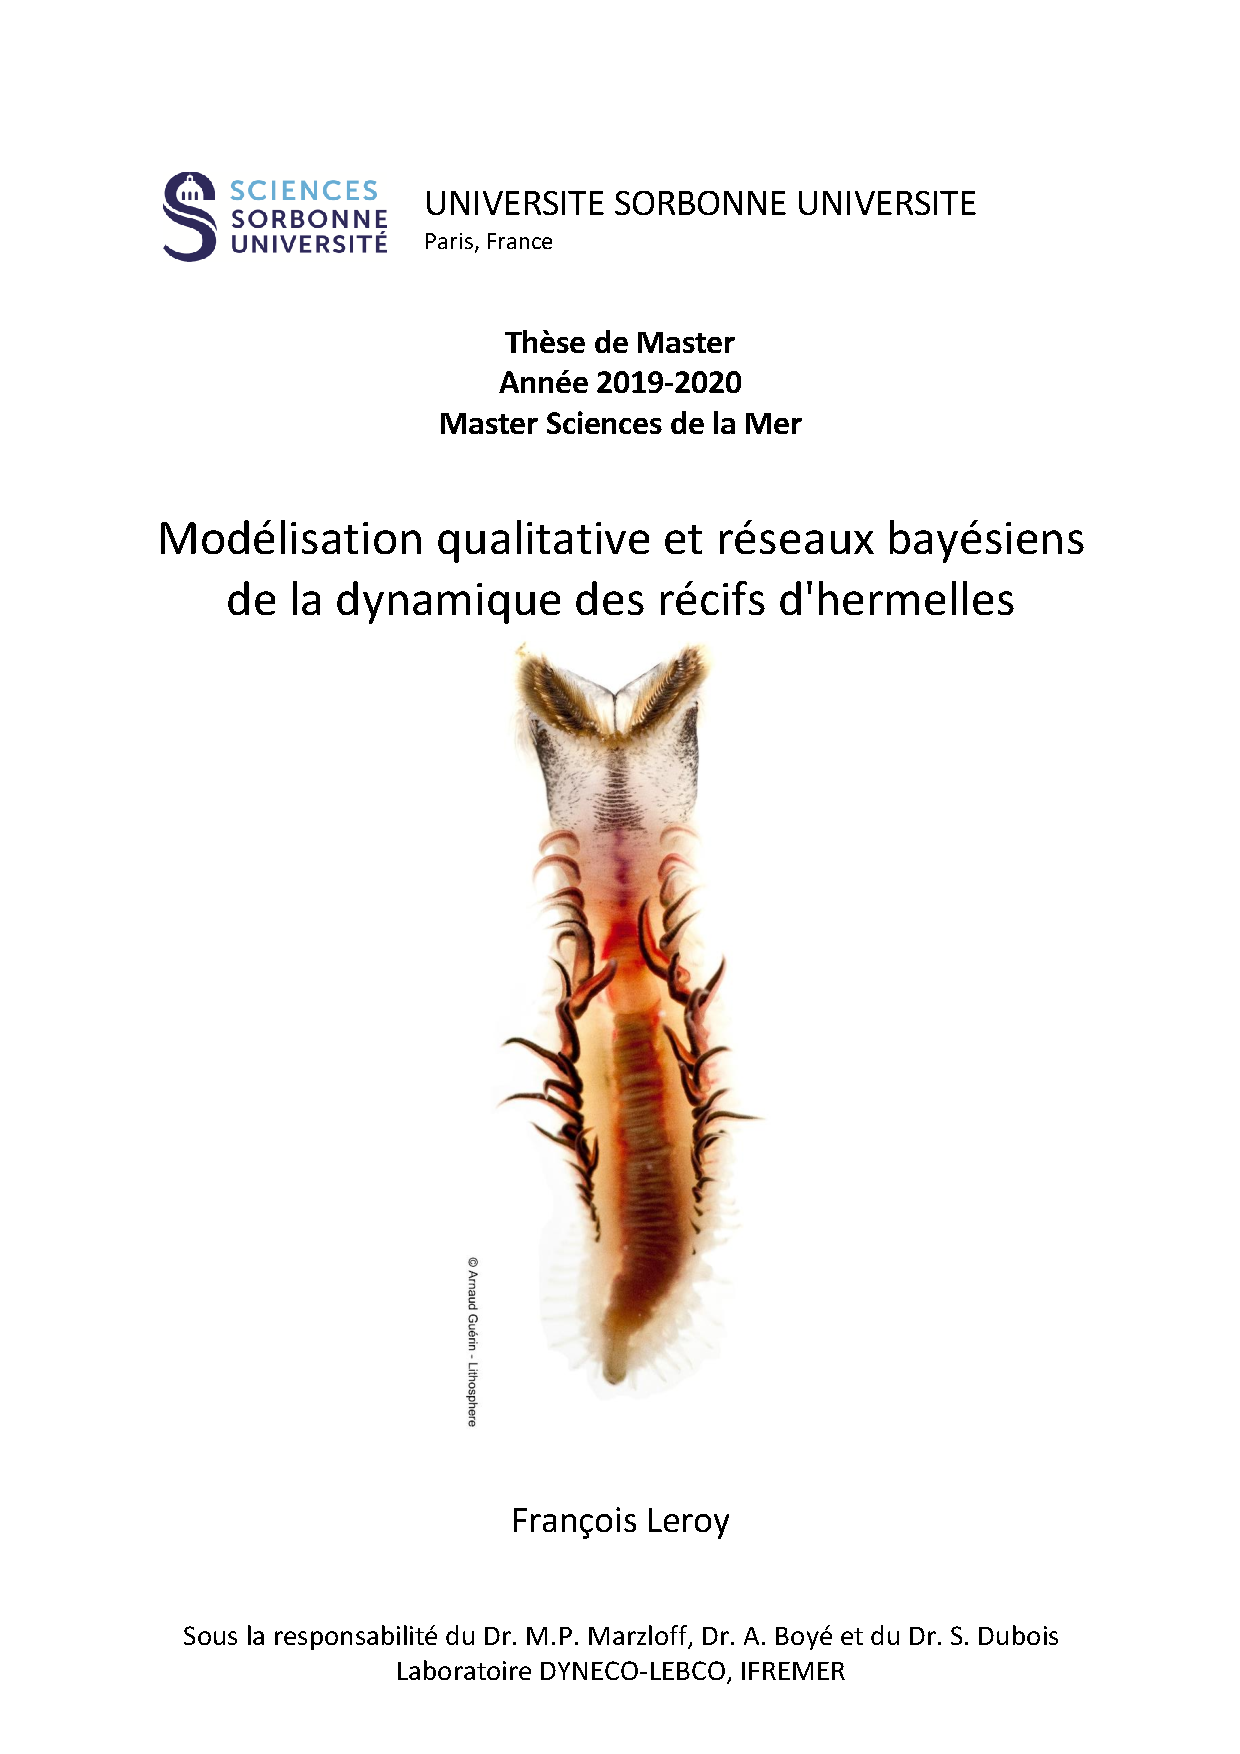
\includepdf[pages = {1}, fitpaper=true]{_assets/coverpage.pdf}

% Roman numbering for content before toc and toc itself
\cleardoublepage 
\pagenumbering{roman}

{
\hypersetup{linkcolor=}
\setcounter{tocdepth}{1}
\tableofcontents
\newpage
}
\vspace{50mm}
\setstretch{1.5}


% Start the arabic numbering at the 1st chapter
\cleardoublepage 
\pagenumbering{arabic}


% The mind, the...
\hypertarget{annotation}{%
\chapter*{Annotation}\label{annotation}}
\addcontentsline{toc}{chapter}{Annotation}

Biodiversity, at the basis of many essentials ecosystem services, is in the process of facing its sixth mass extinction. Although global extinction is unprecedented, there is so far no reason to expect that biodiversity dynamic at lower spatial and temporal scales follow this trend. Thus, links between
spatio-temporal scales and facets of biodiversity (\emph{i.e.} species richness, species diversity, colonization, extinction,
species turnover, etc) need to be fully understood if we want to address this worldwide crisis. So far,
attempts to describe biodiversity changes have been limited mainly by heterogeneity in spatial and
temporal scales that was hardly taken into account by the statistical modelling frameworks.

My PhD project propose to address this flaws in order to understand in more details biodiversity
changes across spatial and temporal scales. Especially, we aim at developing and testing nonparametric
tree-based modelling methods allowing to study the non-linear and interacting effects of
space and time-span on different aspects of biodiversity.

\underline{The specific objectives of my PhD project are:}

\begin{enumerate}
\def\labelenumi{\arabic{enumi}.}
\tightlist
\item
  Modelling and mapping avian species richness changes over Czech Republic across space and time
  scales.
\item
  Decompose the modelled biodiversity to colonization, extinction, species turnover, across spatiotemporal
  scales.
\item
  Estimate the strength of the link between environmental drivers of biodiversity change across
  spatio-temporal scales.
\item
  Apply the previously developed method to other European regions (e.g.~UK, Switzerland, France)
\end{enumerate}

\clearpage

\textbf{PhD candidate:} François Leroy\newline
\textbf{Programme:} Environmental Earth Sciences\newline
\textbf{Department:} \href{https://www.fzp.czu.cz/en/r-9407-departments/r-9471-departments/r-9649-department-of-spatial-sciences}{Applied Geoinformatic and Spatial Planning}\newline
\textbf{Advisor:} \href{http://wp.czu.cz/cs/index.php/?r=1071\&mp=person.info\&idClovek=2155}{doc. Ing. Petra Šímová, Ph.D.}\newline
\textbf{Consultant:} Mgr. \href{http://wp.czu.cz/cs/index.php/?r=1071\&mp=person.info\&idClovek=34772}{Petr Keil}, PhD\newline
\textbf{Beginning of study:} October 2020\newline
\newline

\begingroup
\let\clearpage\relax

\hypertarget{intro}{%
\chapter{Introduction}\label{intro}}

Human life quality is intrinsically linked to ecosystems state that he is living in. Indeed, ecosystems services extend in a large spectrum of mechanisms including nutrient cycle, food production, or climate and water cycle regulation \autocite{pereira_global_2012}. Some of those ecosystem
functions are managed by bird populations such as seed dispersal, controls pests or pollinate plant.
Unfortunately, anthropogenic stressors like habitat loss, over exploitation, pollution or introduction of
invasive species could lead biodiversity to its sixth mass extinction \autocite{barnosky_has_2011}.

While the loss of global biodiversity is unprecedented, current scientific literature has also shown that
temporal trends in local changes of biodiversity can be opposite to trends at larger scales \autocite{chase_species_2019}. Thus, current changes in biodiversity is far more complex than a simple global decrease:
most of the ecosystems undergo alterations of their communities with changes in species composition \autocite{blowes_geography_2019,dornelas_assemblage_2014}.

Typically, biodiversity is considered for a particular taxon (\emph{e.g.} birds, amphibians, reptiles\ldots), but also
according to the spatial scale it is defined by. Here, the term scale refers to the area in which the
biodiversity in considered, also referred hereafter as grain size. So far, it has been assumed that
holding the spatial scale constant when studying biodiversity is mandatory \autocite{whittaker_scale_2001}. As
a matter of fact, it is known that species richness increases with the area considered \autocite{arrhenius_species_1921} and this relationship is approximately linear on a log-log scale (Species-Area Relationship,
SAR). However, this assumption restricts the data accessibility as sampling plans widely differ
according to the species studied, the resources available or, the field conditions. Thus, developing a
method capable of dealing with biodiversity across varying grain size could increase significantly the
data availability. Moreover, it would allow to model biodiversity at different spatial scales than the
ones used in the data. Modelling biodiversity indexes at finer spatial grain size that the data used to
learn the model is referred as \emph{downscaling} biodiversity whilst extrapolating at coarser grain-size is
called \emph{upscaling}.

So far, there are indications that such method can be used. For instance, \textcite{keil_downscaling_2014} and \textcite{keil_downscaling_2013} showed promising downscaling biodiversity models using biodiversity data with different
spatial scales, whilst \textcite{kunin_upscaling_2018} showed that upscaling biodiversity is also possible. Thus, all
the constituents of cross-scales models are known but still need to be gathered and tested. For
instance, \textcite{jarzyna_spatial_2015} used a Bayesian framework to study temporal changes of avian
biodiversity (colonization, extinction, temporal turnover) across scales. However, other approaches
such as parametric Generalized Linear Models (GLM), Generalized Additive Models (GAM) and
Generalized Linear Mixed Model (GLMM) or non-parametric tree based machine learning methods
need to be tested.

\endgroup

\hypertarget{aims}{%
\chapter{Aims}\label{aims}}

The main aim of my PhD will be to test different statistical modeling methods allowing to integrate
cross-scales biodiversity data. This method will allow to model biodiversity facets at various spatial
and temporal grain sizes.

This principal objective can be divided into four sub-objectives:

\begin{enumerate}
\def\labelenumi{\arabic{enumi}.}
\item
  \textbf{I will model temporal dynamics of avian species richness in the Czech Republic across spatio-temporal scales} (\emph{i.e.} grain size ranging from less than 1 Km² to more than 2 000
  Km²). This will allow to map biodiversity over Czech republic at any desired spatial and
  temporal scales. Given the well known Species-Area Relationship \autocites[SAR,][]{arrhenius_species_1921,storch_untangling_2004} and Species-Time Relationship \autocite[STR,][]{white_comparison_2006} we expect to
  see higher species richness at coarser spatial and temporal scales than at finer scales.
  Moreover, we will be able to look at the effect of grain size over biodiversity trends. So far,
  \textcite{chase_species_2019} showed that North American avian biodiversity is largely stable at fine
  scales, but that it tends to increase with spatial scale. Thus, we can expect to observe the same
  trends for the Czech Republic.
\item
  \textbf{I will decompose the modelled biodiversity to colonization, extinction, and species turnover, across spatio-temporal scales.} Indeed, biodiversity dynamic is underlined by
  those ecological processes whose trends can be opposite to the species richness' one \autocite{dornelas_assemblage_2014}. Thus, understanding how they fluctuate according to the spatio-temporal scales
  they are considered will help understand the global biodiversity dynamic. So far, \textcite{jarzyna_spatial_2015} showed that those facets of biodiversity was in general declining with increasing
  spatial grain size for the state of New-York. However the colonization undergoes a slower
  steep. Thus, those trends are also expected to occur with our model for the Czech Republic.
\item
  \textbf{I will estimate the strength of the link between environmental drivers of biodiversity change across spatio-temporal scales.} So far, land use change, habitat loss, or changes in
  climatic conditions are good candidates for such drivers. \textcite{jarzyna_spatial_2015} showed that
  environmental parameters, such as climate change variables (\emph{e.g.} temperatures, pluviometry)
  and landscape variables (\emph{e.g.} elevation, sampling effort), were dependent on the spatial scale
  on the one hand, but also on the metric considered on the other hand (\emph{i.e.} colonization,
  extinction\ldots). Thus, the expectations are more difficult to assess here. What we know is that at
  larger scales (\emph{i.e.} biogeographic or continental), evolutionary processes tend to drive the
  biodiversity patterns \autocite{keil_downscaling_2014}. Climatic and land cover parameters, for their part,
  intervene at scales ranging from tens to hundreds of kilometers. At even finer scales, biotic
  and population dynamics processes are driving.
\item
  \textbf{Once the methods will be validated for the Czech Republic, the logical continuation will be to use it over other European regions (\textit{i.e.} Switzerland, United-Kingdom, Brittany, North America).} The main advantage of looking at other countries is to look at the trend of
  biodiversity facets at larger scales. As for objective 1, we can also expect that the species
  richness trends will tend to increase with spatial scale \autocite{chase_species_2019} whilst, as for
  objective 2, other biodiversity dynamic indexes will decrease \autocite{jarzyna_spatial_2015}.
\end{enumerate}

\hypertarget{method}{%
\chapter{Methodological approach}\label{method}}

\hypertarget{data}{%
\section{Data}\label{data}}

A significant part of this project will consist in \textbf{1)} harvesting, gathering and managing biodiversity
datasets of the aimed taxon (i.e.~birds here) in order to \textbf{2)} use them to model biodiversity facets
across spatial and temporal scales.

Birds represent a key taxon for this problematic as they are various in morphology and colors,
allowing to easily identify and list them. We already have access to high quality avian biodiversity
time series over Czech Republic from the Česka Společnost Ornithologiká \autocite{bejcek_velke_2016}
and the Jednotný Program Sčítání Ptáků \autocite[JPSP,][objective 1 and 2]{reif_population_2006}. Avian biodiversity
will also be studied in other European countries (objective 4) and data for those regions are needed. I
already contacted the Bretagne Vivante association, which handle biodiversity data for Brittany
(\emph{i.e.} French region). It will allow us to access avian biodiversity data for oceanic climate in order to
contrast with the continental climate of the Czech Republic. Other datasets are aimed such as Swiss,
British, Cataloninan or other French biodiversity data. In order to achieve the third objective of this
project, environmental datasets are needed. For instance, the CORINE and HYDE \autocite{goldewijk_hyde_2011} datasets are aimed to access landcover and land use data, respectively. Climatology
timeseries can also be found with Chelsa \autocite{karger_climatologies_2017,karger_data_2018} and WorldClim
datasets \autocite{fick_worldclim_2017}.
Data management represent a significant time consuming part of a modelling project. So far, the
beginning of my PhD consisted mainly into gathering and shaping datasets in order to
be able to analyse and use them to train my models (objective 1). So far, species richness has been computed
from 1973 to 2020 and for areas ranging from less than 1 Km² to more than 2 000 Km². For this, I
used the avian biodiversity atlas data from the Česka Společnost Ornithologiká available at one grainsize
that I aggregated into coarser 2 by 2 and 4 by 4 grain size (\href{https://github.com/FrsLry/IGA_figures/blob/main/maps_IGA.pdf}{Fig. 1}). On the other hand, I managed the
JPSP dataset in a singular way, allowing me to extract species richness from censuses of local points
to censuses of entire transects. Thanks to those, I was able to train my first random forests \textcolor{red}{(see Pilot
results part below)}. Thus, I am already able to shape any biodiversity dataset to use them into the
machine learning framework desired. The next step will be to compute dynamic biodiversity indexes
such as colonization, extinction, temporal turnover and community dissimilarity for objective 2.

\hypertarget{modelling-methods}{%
\section{Modelling methods}\label{modelling-methods}}

Non-parametric tree-based machine learning methods uses variance partitioning to iteratively split
the feature space (features can also be named predictors, covariates, independent or, input variables)
in order to obtain a tree in which one just need to follow the splits to predict an output (\emph{i.e.} the
response variable or dependent variable) such as species richness, colonization, extinction\ldots{}

In order to make a model both understandable and predictive, a balance must be found between
complexity and explicative power \autocite{houlahan_priority_2017}. Thus, using as few covariates as possible to
predict biodiversity is necessary if we want to make the forecasts conveniently and if we want to
discuss our models. We aim to start by using very few covariates such as latitude, longitude, area,
time and time span in order to then add environmental parameters step by step. Tree-based machine
learning methods such as random forests or boosted regression tree \textbf{1)} allows to study the interacting
effect of drivers on the output variable and \textbf{2)} also represent a convenient way of dealing with nonlinear
relationships between the response variable and the covariates. Indeed, \textcite{keil_global_2019}
showed that \textbf{1)} area does have an interacting impact with other environmental and spatial drivers of
biodiversity and \textbf{2)} that this relationship is non linear. Moreover, \textcite{viana_partitioning_2019} showed that
boosted regression trees and random forests predicted ecological indexes more accurately than other
methods. Thus, tree-based modelling methods are totally suited for our purpose. Other parametric
methods such as generalized linear, additive or mixed models (GLM, GAM, GLMM) have already shown
to give satisfying results \autocite{keil_global_2019} and could be used in some of my analysis.

It is important to point out that the proposed methodology here can be applied to any other taxa (\textbf{e.g.}
lepidoptera, large mammals) and any other spatial range (\textbf{e.g.} Europe, North America, South Africa),
which represent the next steps of this project.

\hypertarget{pilot-results}{%
\section{Pilot results}\label{pilot-results}}

So far, I have already been able to produce random forests using only latitude, longitude, area, date, time span and elongation as covariates that explain around 90\% of the species richness variance over
the Czech Republic, which is encouraging (see Fig. 2,
\url{https://github.com/FrsLry/IGA_figures/blob/main/pred_vs_obs.pdf}). An other advantage of the complex
nonparametric models is that you can represent the dependence between the outcome and a
predictor of interest called a marginal plot or partial plot. For instance, in Fig.3
(\url{https://github.com/FrsLry/IGA_figures/blob/main/marginal_plot.pdf}), I represented the influence of the
interacting area and time factors on the species richness for one of my model. In order to validate and
enhance the models performance, the next steps will be to \textbf{1)} perform cross-validation to avoid
overfitting, \textbf{2)} add the adequate environmental parameters and \textbf{3)} connect the local time series from
the JPSP data to the atlas data by using both of them in a single model.

\hypertarget{schedule}{%
\chapter{Schedule}\label{schedule}}

\begin{longtable}[]{@{}lll@{}}
\caption{\label{tab:sched} Planning of the methodological steps of my PhD}\tabularnewline
\toprule
\begin{minipage}[b]{0.21\columnwidth}\raggedright
Start date\strut
\end{minipage} & \begin{minipage}[b]{0.21\columnwidth}\raggedright
End date\strut
\end{minipage} & \begin{minipage}[b]{0.49\columnwidth}\raggedright
Description of the tasks\strut
\end{minipage}\tabularnewline
\midrule
\endfirsthead
\toprule
\begin{minipage}[b]{0.21\columnwidth}\raggedright
Start date\strut
\end{minipage} & \begin{minipage}[b]{0.21\columnwidth}\raggedright
End date\strut
\end{minipage} & \begin{minipage}[b]{0.49\columnwidth}\raggedright
Description of the tasks\strut
\end{minipage}\tabularnewline
\midrule
\endhead
\begin{minipage}[t]{0.21\columnwidth}\raggedright
01/10/2020\strut
\end{minipage} & \begin{minipage}[t]{0.21\columnwidth}\raggedright
01/06/2021\strut
\end{minipage} & \begin{minipage}[t]{0.49\columnwidth}\raggedright
1. Gathering and managing avian biodiversity datasets over Czech Republic (objective 1, 2 and 3). \newline 2. Computing biodiversity indexes (species richness, colonization, extinction, temporal turnover, community similarity) from the data (objective 2 and 3).\strut
\end{minipage}\tabularnewline
\begin{minipage}[t]{0.21\columnwidth}\raggedright
01/06/2021\strut
\end{minipage} & \begin{minipage}[t]{0.21\columnwidth}\raggedright
01/09/2021\strut
\end{minipage} & \begin{minipage}[t]{0.49\columnwidth}\raggedright
Building models for Czech Republic: machine learning models are powerful but need to be parametrized in order to increase predicting power and avoid overfitting. Moreover, I will build my models with significant databases and expect to run long time consuming computing jobs.\strut
\end{minipage}\tabularnewline
\begin{minipage}[t]{0.21\columnwidth}\raggedright
01/01/2022\strut
\end{minipage} & \begin{minipage}[t]{0.21\columnwidth}\raggedright
01/05/2022\strut
\end{minipage} & \begin{minipage}[t]{0.49\columnwidth}\raggedright
1. Testing addition of environmental variables to the random forests in order to increase predictive power (Objective 3).\newline 2. Harvesting and managing avian biodiversity datasets across Europe: objective 4 of this project will be to study biodiversity changes across scales at the European extent. I will have more datasets and management is expected to take more time than for Czech Republic.\strut
\end{minipage}\tabularnewline
\begin{minipage}[t]{0.21\columnwidth}\raggedright
01/05/2022\strut
\end{minipage} & \begin{minipage}[t]{0.21\columnwidth}\raggedright
01/08/2022\strut
\end{minipage} & \begin{minipage}[t]{0.49\columnwidth}\raggedright
Building models for Europe (objective 4): I will build my models with significant databases and expect to run long computing jobs.\strut
\end{minipage}\tabularnewline
\begin{minipage}[t]{0.21\columnwidth}\raggedright
01/08/2022\strut
\end{minipage} & \begin{minipage}[t]{0.21\columnwidth}\raggedright
End of the PhD\strut
\end{minipage} & \begin{minipage}[t]{0.49\columnwidth}\raggedright
1. Building models for North America: Discussions about collaboration with Dr.~Marta Jarzyna is ongoing in order to apply these developed method to North American breeding birds datasets they have access to. \newline 2. Merging the European and North American models will be a good start to look at a the more global biodiversity changes across different continents. \newline 3. Gathering and merging biodiversity datasets from other part of the globe will give us more insights about the main trend of the avian biodiversity changes at worldwide scale.\strut
\end{minipage}\tabularnewline
\bottomrule
\end{longtable}

\hypertarget{benefits}{%
\chapter{Benefits of outcome}\label{benefits}}

My PhD aim at several goals:

\begin{enumerate}
\def\labelenumi{\arabic{enumi}.}
\item
  Better understand the link between spatial and temporal features (\emph{e.g.} latitude, longitude, area, time span) and biodiversity changes.
\item
  Developing a modelling framework (tree-based models) allowing to forecast biodiversity indexes across various space and time scales would help to \textbf{1)} understand and thus \textbf{2)} forecast biodiversity dynamic.
\item
  This method will allow to integrate heterogeneous biodiversity datasets that could usually not be used together with classical statistical models due to their inconsistencies in space and/or time scales. Thus, it will be possible to link local biodiversity datasets (\emph{e.g.} censuses of ornithological associations, participative sciences) to broader ones \autocite[\emph{e.g.} atlas, time-series assemblage such as Biotime database by][]{dornelas_biotime_2018}.
\item
  After focusing on the species richness changes, the link between spatial and temporal scales and the dynamic of other facets of biodiversity (\emph{e.g.} colonization, extinction, \(\beta\) diversity) will be investigated.
\item
  Produce avian biodiversity maps at different spatial and temporal grain sizes over Czech Republic/Europe/North America.
\item
  The parametrized models for birds will give insights on how to apply them to other taxa (\emph{e.g.} lepidoptera, odonata, large mammals\ldots).
\end{enumerate}

\hypertarget{coop}{%
\chapter{Cooperations}\label{coop}}

This project takes part in the broader research project of Dr.~Petr Keil who has been working on the problem of scale-dependent biodiversity change and integration of heterogeneous data for a decade now, and who has published several high-profile publications on these topics. He currently is my PhD supervisor. Petr's expertise will be particularly relevant for tasks requiring advanced statistical modelling, interpretation of the models, and putting the results in a broader macroecological context.

Cooperation is already ongoing with Vladimír Bejček and Karel Šťastný who furnished us time series of avian biodiversity from the Česka Společnost Ornithologiká which were used in the publications of several atlases \autocite[see][]{bejcek_velke_2016}. On the other hand, Dr.~Jiří Reif forwarded me local time series from the Jednotný Program Sčítání Ptáků (JPSP). Their expertise on bird ecologie will be helpful in order to interpret and enhance the outputs of my models.

Finally, discussions with Dr.~Marta Jarzyna (University of Colombus, Ohio) are ongoing in order to work together on applying the methods that I use on Czech Republic and Europe to some American states.As a matter of fact, my results will \textbf{1)} allow to differentiate biodiversity dynamics on the North American and the European continents and \textbf{2)} help to better understand the link between spatio-temporal scales and biodiveristy dynamic by enlarging the databases that I use.

\hypertarget{outcomes}{%
\chapter{Expected outcomes}\label{outcomes}}

\underline{Publications:}

We expect at least 3 publications in journals with high Impact Factor (IF): \textbf{1)} the first one concerning
avian biodiversity indexes dynamic (\emph{i.e.} species richness, colonization, extinction and turnover) across
spatio-temporal scales over Czech Republic (objectives 1 et 2), \textbf{2)} the second one about the
strength of the link between environmental drivers and biodiversity changes across spatio-temporal
scales (objective 3) and \textbf{3)} the third one related to the European avian biodiversity dynamic (objective 4). Publications about North-America and other part of the world can also be expected though the expected outputs still need to be discussed and determined with the foreign teams.

The journals aimed for publication of my PhD project will be the ones focusing on understanding
macroecological patterns and spatio-temporal dynamic in a context of global anthropogenic changes.
Journals interested by testing of new methods and conservation orientated journals will also be aimed.

\textbf{Following are examples of the journals of interest:}

\begin{itemize}
\tightlist
\item
  First quartile journals: Ecography, Diversity and Distributions, Global Change Biology
\item
  Second quartile journals: Ecology and Evolution, Ecological Modeling
\end{itemize}

\underline{Conferences:}

Aimed conferences will be related to ecology and conservation and statistical ecology (\textbf{e.g.} \href{https://www.britishecologicalsociety.org/events/festival-of-ecology/ecology-across-borders-2021/}{Ecology Across Borders 2021}, \href{https://www.esa.org/events/meetings/future-esa-meetings/}{Ecological Society of America}, \href{https://www.cspe.cz/konference/ekologie-2021/}{České společnosti pro ekologii}, \href{https://www.biogeography.org/meetings/}{International Biogeography Society}).\newline\newline

\begingroup
\let\clearpage\relax

\hypertarget{financing}{%
\chapter{Financing}\label{financing}}

My PhD is mainly financed by the \href{https://www.fzp.czu.cz/en/r-9676-news/announcement-of-rees.html}{REES} project until my third year of study. On the other hand, I have been awarded the \href{https://www.fzp.czu.cz/en/r-9409-science-research/r-9531-internal-grant}{IGA grant} for a time period of two years. In order to finance the fourth year of my PhD, one of the grant aimed by Petr Keil is the \href{https://erc.europa.eu/funding/advanced-grants}{advanced grant of the ERC} (European Research Council).

\endgroup


\singlespacing % reset the spacing of the bibliography style
%%%%%%%%%%%%%% Here is the part that I am using for the bibliography to be displayed in the toc
% First step: I define the name and label of the biblio part
\chapter{References}\label{references}
{
% I temporarily redefine the clearpage in order for the bib to not be printed on a new page
\renewcommand{\clearpage}{}
\printbibliography[heading=none] % I delete the default name of the bib
%\printbibliography 
}

\end{document}
